\documentclass[color=usenames,dvipsnames]{beamer}\usepackage[]{graphicx}\usepackage[]{color}
% maxwidth is the original width if it is less than linewidth
% otherwise use linewidth (to make sure the graphics do not exceed the margin)
\makeatletter
\def\maxwidth{ %
  \ifdim\Gin@nat@width>\linewidth
    \linewidth
  \else
    \Gin@nat@width
  \fi
}
\makeatother

\definecolor{fgcolor}{rgb}{0, 0, 0}
\newcommand{\hlnum}[1]{\textcolor[rgb]{0.69,0.494,0}{#1}}%
\newcommand{\hlstr}[1]{\textcolor[rgb]{0.749,0.012,0.012}{#1}}%
\newcommand{\hlcom}[1]{\textcolor[rgb]{0.514,0.506,0.514}{\textit{#1}}}%
\newcommand{\hlopt}[1]{\textcolor[rgb]{0,0,0}{#1}}%
\newcommand{\hlstd}[1]{\textcolor[rgb]{0,0,0}{#1}}%
\newcommand{\hlkwa}[1]{\textcolor[rgb]{0,0,0}{\textbf{#1}}}%
\newcommand{\hlkwb}[1]{\textcolor[rgb]{0,0.341,0.682}{#1}}%
\newcommand{\hlkwc}[1]{\textcolor[rgb]{0,0,0}{\textbf{#1}}}%
\newcommand{\hlkwd}[1]{\textcolor[rgb]{0.004,0.004,0.506}{#1}}%
\let\hlipl\hlkwb

\usepackage{framed}
\makeatletter
\newenvironment{kframe}{%
 \def\at@end@of@kframe{}%
 \ifinner\ifhmode%
  \def\at@end@of@kframe{\end{minipage}}%
  \begin{minipage}{\columnwidth}%
 \fi\fi%
 \def\FrameCommand##1{\hskip\@totalleftmargin \hskip-\fboxsep
 \colorbox{shadecolor}{##1}\hskip-\fboxsep
     % There is no \\@totalrightmargin, so:
     \hskip-\linewidth \hskip-\@totalleftmargin \hskip\columnwidth}%
 \MakeFramed {\advance\hsize-\width
   \@totalleftmargin\z@ \linewidth\hsize
   \@setminipage}}%
 {\par\unskip\endMakeFramed%
 \at@end@of@kframe}
\makeatother

\definecolor{shadecolor}{rgb}{.97, .97, .97}
\definecolor{messagecolor}{rgb}{0, 0, 0}
\definecolor{warningcolor}{rgb}{1, 0, 1}
\definecolor{errorcolor}{rgb}{1, 0, 0}
\newenvironment{knitrout}{}{} % an empty environment to be redefined in TeX

\usepackage{alltt}
%\documentclass[color=usenames,dvipsnames,handout]{beamer}

\usepackage[roman]{../lectures}
%\usepackage[sans]{../lectures}


\hypersetup{pdfpagemode=UseNone,pdfstartview={FitV}}


\title{Lecture 2 -- Basic statistical models}
\author{Richard Chandler}


% Load function to compile and open PDF


% Compile and open PDF







%<<knitr-setup,include=FALSE,purl=FALSE>>=
%##opts_chunk$set(comment=NA)
%@


%% New command for inline code that isn't to be evaluated
\definecolor{inlinecolor}{rgb}{0.878, 0.918, 0.933}
\newcommand{\inr}[1]{\colorbox{inlinecolor}{\texttt{#1}}}
\IfFileExists{upquote.sty}{\usepackage{upquote}}{}
\begin{document}

% This would affect all code boxes. Not a good idea.
% \setlength\fboxsep{0pt}



\begin{frame}[plain]
  \LARGE
%  \maketitle
  \centering
  {\huge Lecture 2 -- Refresher of basic statistical models} \\
  {\color{default} \rule{\textwidth}{0.1pt}}
  \vfill
  \large
  WILD(FISH) 8390 \\
  Estimation of Fish and Wildlife Population Parameters \\
  \vfill
  \large
  Richard Chandler \\
  University of Georgia \\
\end{frame}




\section{Linear models}


\begin{frame}[plain]
  \frametitle{Today's Topics}
  \Large
  \only<1>{\tableofcontents}%[hideallsubsections]}
  \only<2 | handout:0>{\tableofcontents[currentsection]}%,hideallsubsections]}
\end{frame}




\begin{frame}
  \frametitle{Linear models}
%  \small
  All ANOVAs and fixed-effects regression models are linear models \\
  \vspace{12pt}
  You must understand linear models before you can apply more advanced
  models such as GLMs, GAMS, hierarchical models etc\dots  
  \vfill
  \centering
  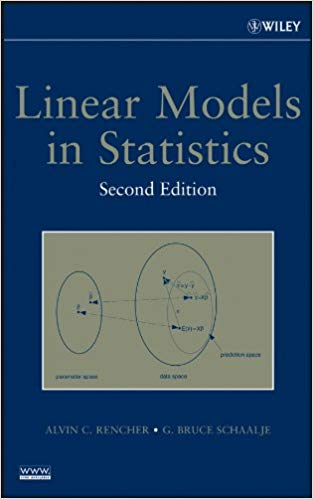
\includegraphics[width=0.25\textwidth]{figure/Rencher_Schaal_book} \hspace{1cm}
  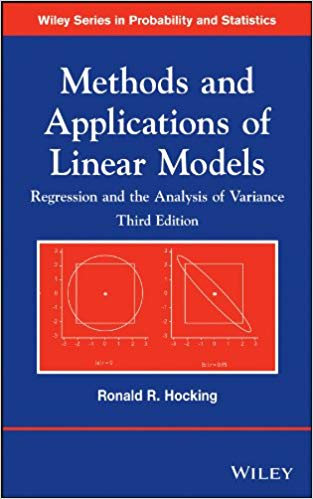
\includegraphics[width=0.25\textwidth]{figure/Hocking_book} \\
\end{frame}


\begin{frame}
  \frametitle{Simple linear regression}
  Simple linear regression is the most basic linear model.
  \[
    y_i = \beta_0 + \beta_1 x_i + \varepsilon_i \qquad \qquad
    \varepsilon_i \sim \mathrm{Norm}(0, \sigma^2)
  \]
  \vspace{-6pt}
  \pause
  \begin{columns}[T]
    \begin{column}{0.5\textwidth}
      $y$ is variously called:
      \begin{itemize}
        \item response variable
        \item outcome variable
        \item dependent variable
      \end{itemize}
    \end{column}
    \pause
    \begin{column}{0.5\textwidth}
      It's worse for $x$
      \begin{itemize}
        \item predictor variable
        \item explanatory variable
        \item independent variable
        \item covariate
        \item exposure
      \end{itemize}
    \end{column}
  \end{columns}
  \pause
  \vfill
  We observe $x$ and $y$. \\
  \vfill
  We'd like to estimate $\beta_0$ and $\beta_1$, called the ``coefficients''. \\
  \pause
  \vfill
  The $\{\varepsilon_i\}$ are residuals. $\sigma^2$ is their variance.
\end{frame}



\begin{frame}[fragile]
  \frametitle{Probability distributions}
  Check out Heather Gaya's awesome Shiny App: \\
  \vfill
  \centering
  \href{ % Highlighting gets messed up if on 1 line
    https://insects.shinyapps.io/Probability_Dists/
  }{
    \large
    \color{blue}
    {https://insects.shinyapps.io/Probability\_Dists/} 
  } \\
  \vfill
  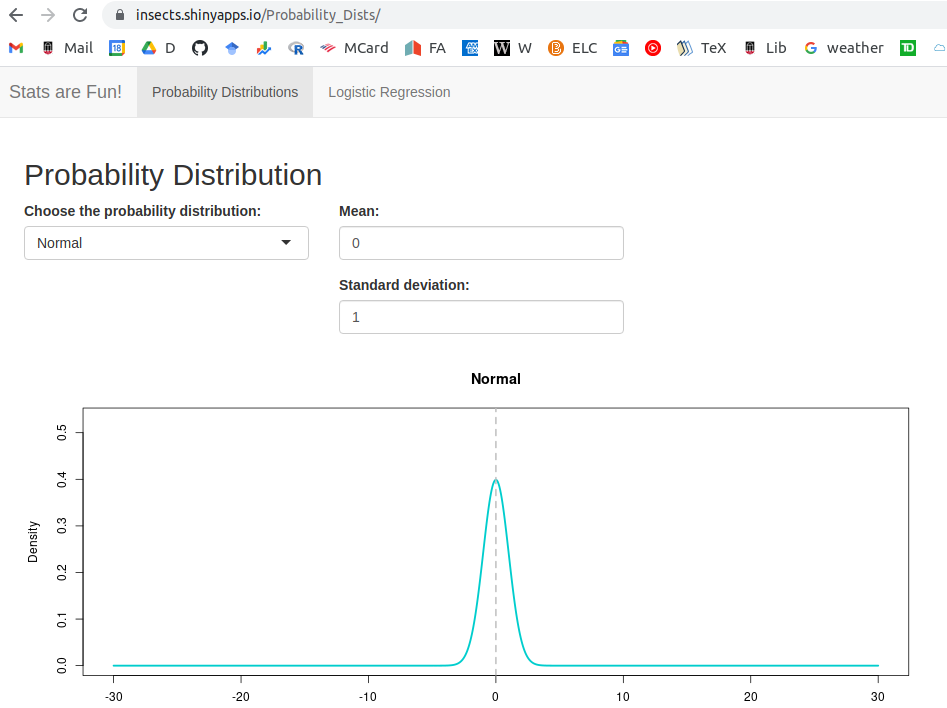
\includegraphics[width=0.7\textwidth]{figs/probDists} \\
\end{frame}






\begin{frame}[fragile]
  \frametitle{Simple linear regression example}
  Suppose your data look like this:
\begin{knitrout}\scriptsize
\definecolor{shadecolor}{rgb}{0.878, 0.918, 0.933}\color{fgcolor}\begin{kframe}
\begin{alltt}
\hlstd{x} \hlkwb{<-} \hlkwd{c}\hlstd{(}\hlnum{0.30}\hlstd{,} \hlnum{0.91}\hlstd{,} \hlnum{0.89}\hlstd{,} \hlnum{0.24}\hlstd{,} \hlnum{0.77}\hlstd{,} \hlnum{0.56}\hlstd{,} \hlnum{0.59}\hlstd{,} \hlnum{0.92}\hlstd{,} \hlnum{0.81}\hlstd{,} \hlnum{0.59}\hlstd{)}
\hlstd{y} \hlkwb{<-} \hlkwd{c}\hlstd{(}\hlnum{0.08}\hlstd{,} \hlnum{0.59}\hlstd{,} \hlnum{0.18}\hlstd{,} \hlnum{0.17}\hlstd{,} \hlnum{0.42}\hlstd{,} \hlnum{0.71}\hlstd{,} \hlnum{0.49}\hlstd{,} \hlnum{0.75}\hlstd{,} \hlnum{0.46}\hlstd{,} \hlnum{0.04}\hlstd{)}
\end{alltt}
\end{kframe}
\end{knitrout}
\begin{columns}
  \begin{column}{0.5\textwidth}
\begin{knitrout}
\definecolor{shadecolor}{rgb}{0.878, 0.918, 0.933}\color{fgcolor}
\includegraphics[width=\maxwidth]{figure/slr-viz-1} 
\end{knitrout}
  \end{column}
  \pause
  \begin{column}{0.5\textwidth}
    Classical inference is easy:
\begin{knitrout}\scriptsize
\definecolor{shadecolor}{rgb}{0.878, 0.918, 0.933}\color{fgcolor}\begin{kframe}
\begin{alltt}
\hlkwd{lm}\hlstd{(y}\hlopt{~}\hlstd{x)}
\end{alltt}
\begin{verbatim}
## 
## Call:
## lm(formula = y ~ x)
## 
## Coefficients:
## (Intercept)            x  
##     0.02742      0.54951
\end{verbatim}
\end{kframe}
\end{knitrout}
  \end{column}
\end{columns}
\end{frame}


\begin{frame}
  \frametitle{Bayesian inference with JAGS}
  We will use JAGS and the R packages `rjags' and `jagsUI'.
  JAGS can be downloaded here:  \\
  \centering
  \vfill
  \href{
    https://sourceforge.net/projects/mcmc-jags/files/}{
    \large
    \color{blue}
    https://sourceforge.net/projects/mcmc-jags/files/
  } \\
  \pause
  \vfill
  \flushleft
  The basic steps of Bayesian analysis with JAGS are:
  \begin{enumerate}%[<+->]
    \item Write a model in the BUGS language in a text file
    \item Put data in a named list
    \item Create a function to generate random initial values
    \item Specify the parameters you want to monitor
    \item Use MCMC to draw posterior samples
    \item Use posterior samples for inference and prediction
  \end{enumerate}
\end{frame}





\begin{frame}[fragile]
  \frametitle{Simple (Bayesian) linear regression}
  \small
  The model is in a text file named {\tt lm.jag} \\
\begin{knitrout}\scriptsize
\definecolor{shadecolor}{rgb}{0.878, 0.918, 0.933}\color{fgcolor}\begin{kframe}
\begin{verbatim}
model {

# Priors
## dnorm arguments: mean and precision (1/variance)
beta0 ~ dnorm(0, 0.1)  
beta1 ~ dnorm(0, 0.1)
sigmaSq ~ dunif(0, 2)

## Model for the data
for(i in 1:n) {
  y[i] ~ dnorm(beta0 + beta1*x[i], 1/sigmaSq)
  }

}
\end{verbatim}
\end{kframe}
\end{knitrout}
\pause
\vfill
Now, put the data in a list and pick some initial values
\begin{knitrout}
\definecolor{shadecolor}{rgb}{0.878, 0.918, 0.933}\color{fgcolor}\begin{kframe}
\begin{alltt}
\hlstd{jd.lm} \hlkwb{<-} \hlkwd{list}\hlstd{(}\hlkwc{x}\hlstd{=x,} \hlkwc{y}\hlstd{=y,} \hlkwc{n}\hlstd{=}\hlkwd{length}\hlstd{(y))}
\hlstd{ji.lm} \hlkwb{<-} \hlkwa{function}\hlstd{()} \hlkwd{c}\hlstd{(}\hlkwc{beta0}\hlstd{=}\hlnum{0}\hlstd{,} \hlkwc{beta1}\hlstd{=}\hlnum{0}\hlstd{,} \hlkwc{sigmaSq}\hlstd{=}\hlnum{1}\hlstd{)}
\hlstd{jp.lm} \hlkwb{<-} \hlkwd{c}\hlstd{(}\hlstr{"beta0"}\hlstd{,} \hlstr{"beta1"}\hlstd{,} \hlstr{"sigmaSq"}\hlstd{)}
\end{alltt}
\end{kframe}
\end{knitrout}
\end{frame}


\begin{frame}[fragile]
  \frametitle{Simple (Bayesian) linear regression}
  Use MCMC to draw posterior samples:
\begin{knitrout}\scriptsize
\definecolor{shadecolor}{rgb}{0.878, 0.918, 0.933}\color{fgcolor}\begin{kframe}
\begin{alltt}
\hlkwd{library}\hlstd{(jagsUI)}
\hlstd{js.lm} \hlkwb{<-} \hlkwd{jags.basic}\hlstd{(}\hlkwc{data}\hlstd{=jd.lm,} \hlkwc{inits}\hlstd{=ji.lm,} \hlkwc{parameters.to.save}\hlstd{=jp.lm,}
                    \hlkwc{model.file}\hlstd{=}\hlstr{"lm.jag"}\hlstd{,} \hlkwc{n.chains}\hlstd{=}\hlnum{1}\hlstd{,} \hlkwc{n.iter}\hlstd{=}\hlnum{1000}\hlstd{)}
\end{alltt}
\end{kframe}
\end{knitrout}
\pause
\begin{columns}
  \begin{column}{0.55\textwidth}
    Summarize the posterior samples:
\begin{knitrout}\scriptsize
\definecolor{shadecolor}{rgb}{0.878, 0.918, 0.933}\color{fgcolor}\begin{kframe}
\begin{alltt}
\hlkwd{round}\hlstd{(}\hlkwd{summary}\hlstd{(js.lm)}\hlopt{$}\hlstd{quant,} \hlnum{2}\hlstd{)}
\end{alltt}
\begin{verbatim}
##           2.5%   25%  50%  75% 97.5%
## beta0    -0.64 -0.16 0.02 0.21  0.71
## beta1    -0.44  0.28 0.56 0.81  1.49
## deviance -2.59 -1.01 1.20 4.37 14.45
## sigmaSq   0.03  0.05 0.08 0.14  0.45
\end{verbatim}
\end{kframe}
\end{knitrout}
\pause
  \end{column}
  \begin{column}{0.45\textwidth}
\begin{knitrout}
\definecolor{shadecolor}{rgb}{0.878, 0.918, 0.933}\color{fgcolor}
\includegraphics[width=\maxwidth]{figure/lm-jags-viz-1} 
\end{knitrout}
  \end{column}
\end{columns}
\end{frame}




\begin{frame}
  \frametitle{Linear models}
    A more general depiction of linear models:

\[
y_i = \beta_0 + \beta_1 x_{i1} + \beta_2 x_{i2} + \ldots + \beta_p x_{ip} + \varepsilon_i
\]

where the $\beta$'s are coefficients, and the $x$ values are predictor
variables (or dummy variables for categorical predictors). %\pause
The residuals are assumed to be normally distributed:

\[
  \varepsilon_i \sim \mathrm{Norm}(0, \sigma^2)
\]

\pause

\vfill %\vspace{0.5cm}

% {\bf This equation is often expressed in matrix notation as:}

% \[
% {\bf y} = {\bf X} {\bm{\beta}} + {\bm \varepsilon}
% \]

% where $\bf X$ is a \alert{design matrix} and $\bm{\beta}$ is a
% vector of coefficients. %\pause More on matrix notation later\dots
Linear models can also be written this way:
\begin{gather*}
  \mu_i = \beta_0 + \beta_1 x_{i1} + \beta_2 x_{i2} + \cdots + \beta_p x_{ip} \\
  y_i \sim \mathrm{Normal}(\mu_i, \sigma^2)
\end{gather*}

\end{frame}




\begin{frame}
  \frametitle{Interpreting the $\beta$'s}
You must be able to interpret the $\beta$
coefficients for {\it any model} that you fit to your data.
\pause
\vfill
A linear model might have dozens of continuous and categorical
predictors variables, with dozens of associated $\beta$ coefficients.
\pause
\vfill
%% Key points for interpretting $\beta$'s:
%% \begin{itemize}
%%   \item For continuous explano
%% \end{itemize}
Linear models can also include polynomial terms and interactions
\end{frame}


\begin{frame}[fragile]
  \frametitle{Interpreting the $\beta$'s}
  \small 
  The intercept $\beta_0$ is the expected value of $y$, when all $x=0$ \\
  \pause
  \vfill
  If $x_1$ is a {\bf continuous} explanatory variable: %, $\beta$ is
  \begin{itemize}
    \item $\beta_1$ can usually be interpreted as a \textit{slope}
      parameter
    \item In this case, $\beta_1$ is the
      change in $y$ resulting from a 1 unit change in $x_1$ (while
      holding the other predictors constant)
    \end{itemize}
\pause
\vfill

\centering
\begin{columns}
  \begin{column}{0.5\textwidth}
\begin{knitrout}\tiny
\definecolor{shadecolor}{rgb}{0.878, 0.918, 0.933}\color{fgcolor}\begin{kframe}
\begin{alltt}
\hlkwd{lm}\hlstd{(y}\hlopt{~}\hlstd{x1)}
\end{alltt}
\begin{verbatim}
## 
## Call:
## lm(formula = y ~ x1)
## 
## Coefficients:
## (Intercept)           x1  
##       9.116        1.032
\end{verbatim}
\end{kframe}
\end{knitrout}
  \end{column}
  \begin{column}{0.4\textwidth}
  \includegraphics[width=\textwidth]{figure/linmod-1} \\
  \end{column}
\end{columns}
\end{frame}




\begin{frame}[fragile]
  \frametitle{\small Interpreting $\beta$'s for categorical explanatory variables}
  Things are more complicated for {\bf categorical} explanatory
  variables (i.e., factors) because they must be converted to dummy
  variables
  \pause
  \vfill
  There are many ways of creating dummy variables
  \pause
  \vfill
%  For a {\bf categorical} explanatory variable %, $\beta$ is
  In \R, the default method for creating dummy variables from
  unordered factors works like
  this: %unordered factors is called \inr{"contr.treatment"}
  \begin{itemize}
    \item One level of the factor is treated as a \alert{reference level}
    \item The reference level is associated with the intercept
    \item The $\beta$ coefficients for the other levels of the factor
      are differences from the reference level
  \end{itemize}
%   \pause
%   \vfill
%   The default method corresponds to:
% <<contr-trt,size='small'>>=
% options(contrasts=c("contr.treatment","contr.poly"))
% @
\end{frame}





\begin{frame}[fragile]
  \frametitle{\small Interpreting $\beta$'s for categorical explanatory variables}
\small 

\centering
%\begin{columns}
%  \begin{column}{0.5\textwidth}
\begin{knitrout}\tiny
\definecolor{shadecolor}{rgb}{0.878, 0.918, 0.933}\color{fgcolor}\begin{kframe}
\begin{alltt}
\hlkwd{lm}\hlstd{(y}\hlopt{~}\hlstd{xc)}
\end{alltt}
\begin{verbatim}
## 
## Call:
## lm(formula = y ~ xc)
## 
## Coefficients:
## (Intercept)          xc2          xc3          xc4  
##     10.2147       0.9994      -1.3335       0.6294
\end{verbatim}
\end{kframe}
\end{knitrout}
%  \end{column}
%  \begin{column}{0.4\textwidth}
  \includegraphics[width=0.5\textwidth]{figure/linmod-xc-1} \\
%  \end{column}
%\end{columns}
\end{frame}





% \begin{frame}[fragile]
%   \frametitle{\small Interpretting $\beta$'s for categorical explantory variables}
%   Another common method for creating dummy variables results in
%   $\beta$'s that can be interpretted as the $\alpha$'s from the
%   additive models that we saw earlier in the class.
%   \pause
%   \vfill
%   With this method:
%   \begin{itemize}
%     \item The $\beta$ associated with each level of the factor is the
%       difference from the intercept
%     \item The intercept can be interpetted as the grand mean if the
%       continuous variables have been centered
%     \item One of the levels of the factor will not be displayed
%       because it is redundant when the intercept is estimated
%   \end{itemize}
%   \pause
%   \vfill
%   This method corresponds to:
% <<contr-sum,size='small',eval=FALSE>>=
% options(contrasts=c("contr.sum","contr.poly"))
% @
% \end{frame}



% \subsection{Example}



\begin{frame}
  \frametitle{Ruffed grouse data}
  \centering
  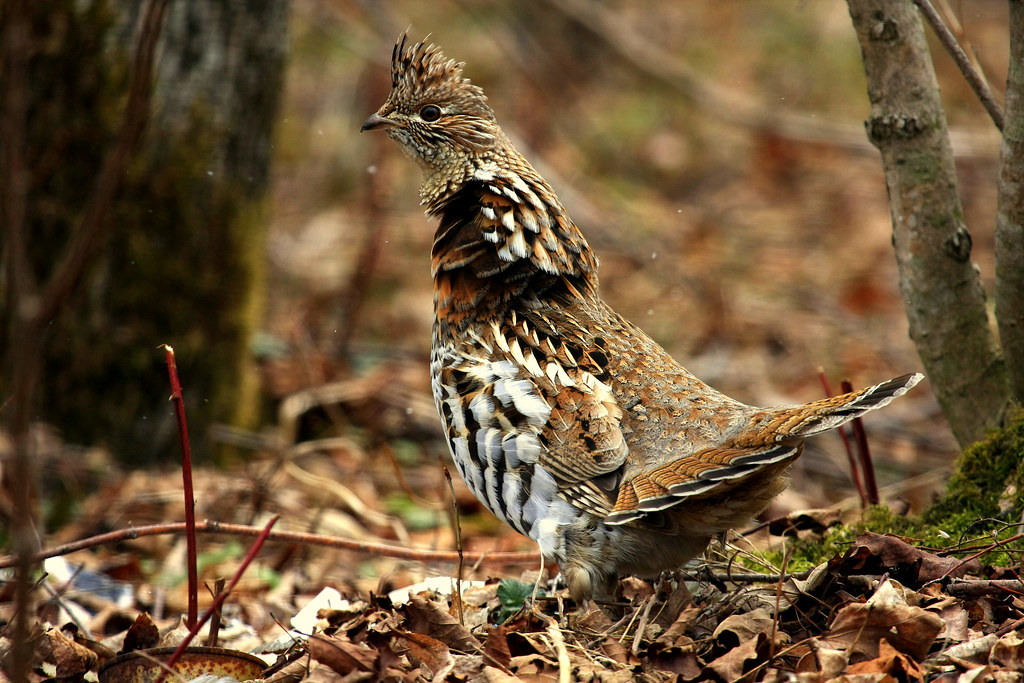
\includegraphics[width=\textwidth]{figs/RUGR}
\end{frame}



\begin{frame}
  \frametitle{Ruffed grouse data}
  \centering
  \includegraphics[width=\textwidth]{figs/grouse_map_locs}
\end{frame}




\begin{frame}[fragile]
  \frametitle{Ruffed grouse data}
  \small
  Import the data and convert \inr{route} and \inr{utmZone} to
  factors. 
\begin{knitrout}\tiny
\definecolor{shadecolor}{rgb}{0.878, 0.918, 0.933}\color{fgcolor}\begin{kframe}
\begin{alltt}
\hlstd{grouse.data} \hlkwb{<-} \hlkwd{read.csv}\hlstd{(}\hlstr{"grouse_data_glm.csv"}\hlstd{,} \hlkwc{row.names}\hlstd{=}\hlnum{1}\hlstd{)}
\hlstd{grouse.data}\hlopt{$}\hlstd{route} \hlkwb{<-} \hlkwd{factor}\hlstd{(grouse.data}\hlopt{$}\hlstd{route)}
\hlstd{grouse.data}\hlopt{$}\hlstd{utmZone} \hlkwb{<-} \hlkwd{factor}\hlstd{(grouse.data}\hlopt{$}\hlstd{utmZone)}
\hlkwd{str}\hlstd{(grouse.data)}
\end{alltt}
\begin{verbatim}
## 'data.frame':	579 obs. of  7 variables:
##  $ abundance: int  0 0 0 0 0 0 0 0 0 0 ...
##  $ presence : int  0 0 0 0 0 0 0 0 0 0 ...
##  $ route    : Factor w/ 54 levels "14","15","16",..: 30 30 30 30 30 30 30 30 30 30 ...
##  $ utmE     : int  760582 760582 760582 760582 760582 760582 760582 760582 760582 760582 ...
##  $ utmN     : int  3873068 3873068 3873068 3873068 3873068 3873068 3873068 3873068 3873068 3873068 ...
##  $ utmZone  : Factor w/ 2 levels "16S","17S": 1 1 1 1 1 1 1 1 1 1 ...
##  $ elevation: num  575 575 575 575 575 ...
\end{verbatim}
\end{kframe}
\end{knitrout}
\end{frame}



\begin{frame}[fragile]
  \frametitle{Grouse data}
  Fit a linear model to the abundance data
\begin{knitrout}\scriptsize
\definecolor{shadecolor}{rgb}{0.878, 0.918, 0.933}\color{fgcolor}\begin{kframe}
\begin{alltt}
\hlstd{fm1} \hlkwb{<-} \hlkwd{lm}\hlstd{(abundance} \hlopt{~} \hlstd{elevation} \hlopt{+} \hlstd{utmZone, grouse.data)}
\hlkwd{summary}\hlstd{(fm1)}
\end{alltt}
\begin{verbatim}
## 
## Call:
## lm(formula = abundance ~ elevation + utmZone, data = grouse.data)
## 
## Residuals:
##      Min       1Q   Median       3Q      Max 
## -0.06062 -0.05363 -0.02424 -0.01492  1.94864 
## 
## Coefficients:
##               Estimate Std. Error t value Pr(>|t|)  
## (Intercept)  3.652e-02  3.585e-02   1.019   0.3088  
## elevation    3.158e-05  5.946e-05   0.531   0.5955  
## utmZone17S  -4.506e-02  2.204e-02  -2.044   0.0414 *
## ---
## Signif. codes:  0 '***' 0.001 '**' 0.01 '*' 0.05 '.' 0.1 ' ' 1
## 
## Residual standard error: 0.2087 on 576 degrees of freedom
## Multiple R-squared:  0.00866,	Adjusted R-squared:  0.005218 
## F-statistic: 2.516 on 2 and 576 DF,  p-value: 0.08169
\end{verbatim}
\end{kframe}
\end{knitrout}
\end{frame}




\begin{frame}[fragile]
  \frametitle{Grouse data}
  Predict grouse abundance at a sequence of elevations for
  each region (east or west side) of the study area. \\
  \vfill
  First, create a new \inr{data.frame} with the explanatory values of
  interest.
\begin{knitrout}\scriptsize
\definecolor{shadecolor}{rgb}{0.878, 0.918, 0.933}\color{fgcolor}\begin{kframe}
\begin{alltt}
\hlstd{elev.min} \hlkwb{<-} \hlkwd{min}\hlstd{(grouse.data}\hlopt{$}\hlstd{elevation)}
\hlstd{elev.max} \hlkwb{<-} \hlkwd{max}\hlstd{(grouse.data}\hlopt{$}\hlstd{elevation)}
\hlstd{seq.length} \hlkwb{<-} \hlnum{20} \hlcom{## Determines how smooth the function looks in GLMs }
\hlstd{elev.seq} \hlkwb{<-} \hlkwd{seq}\hlstd{(}\hlkwc{from}\hlstd{=elev.min,} \hlkwc{to}\hlstd{=elev.max,} \hlkwc{length.out}\hlstd{=seq.length)}
\hlstd{pred.data.west} \hlkwb{<-} \hlkwd{data.frame}\hlstd{(}\hlkwc{elevation}\hlstd{=elev.seq,} \hlkwc{utmZone}\hlstd{=}\hlstr{"16S"}\hlstd{)}
\hlstd{pred.data.east} \hlkwb{<-} \hlkwd{data.frame}\hlstd{(}\hlkwc{elevation}\hlstd{=elev.seq,} \hlkwc{utmZone}\hlstd{=}\hlstr{"17S"}\hlstd{)}
\end{alltt}
\end{kframe}
\end{knitrout}
\pause
\vfill
  Now get the predictions.
\begin{knitrout}\scriptsize
\definecolor{shadecolor}{rgb}{0.878, 0.918, 0.933}\color{fgcolor}\begin{kframe}
\begin{alltt}
\hlstd{pred.west} \hlkwb{<-} \hlkwd{predict}\hlstd{(fm1,} \hlkwc{newdata}\hlstd{=pred.data.west,} \hlkwc{se}\hlstd{=}\hlnum{TRUE}\hlstd{)}
\hlstd{pred.east} \hlkwb{<-} \hlkwd{predict}\hlstd{(fm1,} \hlkwc{newdata}\hlstd{=pred.data.east,} \hlkwc{se}\hlstd{=}\hlnum{TRUE}\hlstd{)}
\end{alltt}
\end{kframe}
\end{knitrout}
\end{frame}



\begin{frame}[fragile]
  \frametitle{Grouse data}
\begin{knitrout}\scriptsize
\definecolor{shadecolor}{rgb}{0.878, 0.918, 0.933}\color{fgcolor}\begin{kframe}
\begin{alltt}
\hlkwd{plot}\hlstd{(abundance} \hlopt{~} \hlstd{elevation,} \hlkwc{data}\hlstd{=grouse.data,} \hlkwc{ylim}\hlstd{=}\hlkwd{c}\hlstd{(}\hlnum{0}\hlstd{,}\hlnum{2}\hlstd{))}
\hlkwd{lines}\hlstd{(elev.seq, pred.west}\hlopt{$}\hlstd{fit,} \hlkwc{col}\hlstd{=}\hlstr{"blue"}\hlstd{,} \hlkwc{lwd}\hlstd{=}\hlnum{2}\hlstd{)}
\hlkwd{lines}\hlstd{(elev.seq, pred.east}\hlopt{$}\hlstd{fit,} \hlkwc{col}\hlstd{=}\hlstr{"grey"}\hlstd{,} \hlkwc{lwd}\hlstd{=}\hlnum{2}\hlstd{)}
\hlkwd{legend}\hlstd{(}\hlnum{900}\hlstd{,} \hlnum{2}\hlstd{,} \hlkwd{c}\hlstd{(}\hlstr{"West"}\hlstd{,} \hlstr{"East"}\hlstd{),} \hlkwc{lty}\hlstd{=}\hlnum{1}\hlstd{,} \hlkwc{col}\hlstd{=}\hlkwd{c}\hlstd{(}\hlstr{"blue"}\hlstd{,}\hlstr{"grey"}\hlstd{),} \hlkwc{lwd}\hlstd{=}\hlnum{2}\hlstd{)}
\end{alltt}
\end{kframe}

{\centering \includegraphics[width=0.85\textwidth]{figure/grouse-pred-plot-1} 

}


\end{knitrout}
\end{frame}



\section{Generalized linear models}



\begin{frame}[plain]
  \frametitle{Outline}
  \Large
  \tableofcontents[currentsection]
\end{frame}




\begin{frame}
  \frametitle{Generalized linear models (GLMs)}
  \large
  \uncover<1->{{\bf Benefits of generalized linear models}}
  \begin{itemize}%[<+->]
    \item<2-> The residuals don't have to be normally distributed
    \item<3-> The response variable can be binary, integer,
      strictly-positive, etc...
    \item<4-> The variance is not assumed to be constant
    \item<5-> Useful for manipulative experiments or observational
      studies, just like linear models.
  \end{itemize}
  \vfill
  \uncover<6->{
  {\bf Examples}
  \begin{itemize}
    \item Presence-absence studies
    \item Studies of survival
    \item Seed germination studies
  \end{itemize}
  }
\end{frame}



\begin{frame}
  \frametitle{Two important GLMs}
  {\bf Logistic regression \\}
  \begin{itemize}
    \item The response variable is usually binary and modeled with a
      binomial distribution
    \item The probability of success is usually a logit-linear
      model
  \end{itemize}
  \pause
  \vfill
  {\bf Poisson regression \\}
  \begin{itemize}
    \item The response variable is a non-negative integer modeled with
      a Poisson distribution
    \item The expected count is usually modeled with a log-linear
      model
  \end{itemize}
  \vfill
\end{frame}



\begin{frame}
  \frametitle{From linear to generalized linear}
  {\bf Linear model}
  \begin{gather*}
    \mu_i = \beta_0 + \beta_1 x_{i1} + \beta_2 x_{i2} + \cdots + \beta_p x_{ip} \\
    y_i \sim \mathrm{Normal}(\mu_i, \sigma^2)
  \end{gather*}
  \pause
  \vfill
  {\bf Generalized Linear model}
  \begin{gather*}
    g(\mu_i) = \beta_0 + \beta_1 x_{i1} + \beta_2 x_{i2} + \cdots + \beta_p x_{ip} \\
    y_i \sim f(\mu_i)
  \end{gather*}
  \pause
  {\bf where} \\
  $g$ is a link function, such as the log or logit link \\
  \pause
  $f$ is a probability distribution such as the binomial or Poisson
%  that determines (usually) the variance %(there is no $\sigma^2$ parameter!)
\end{frame}


\begin{frame}
  \frametitle{Alternative representations}
  {\bf This:}
  \begin{gather*}
    g(\mu_i) = \beta_0 + \beta_1 x_{i1} + \beta_2 x_{i2} + \cdots + \beta_p x_{ip} \\
    y_i \sim f(\mu_i)
  \end{gather*}
  \pause
  {\bf Is the same as this:}
  \begin{gather*}
    \mu_i = g^{-1}(\beta_0 + \beta_1 x_{i1} + \beta_2 x_{i2} + \cdots + \beta_p x_{ip}) \\
    y_i \sim f(\mu_i)
  \end{gather*}
  % \pause
  % {\bf Is the same as this:}
  % \begin{gather*}
  %   g(\mu_i) = {\bf X}{\bm \beta} \\
  %   y_i \sim f(\mu_i)
  % \end{gather*}
\end{frame}


\begin{frame}
  \frametitle{Link functions}
%  \begin{itemize}[<+->]
%    \item
  An inverse link function ($g^{-1}$) transforms values from the $(-\infty,\infty)$
  scale to the scale of interest, such as $(0,1)$ for probabilities  \\
  \pause
  \vfill
%    \item
  The link function ($g$) does the reverse \\
%    \item
%  \pause
%  \vfill
%  The two link functions that you will see most often are the
%      ``logit'' and ``log'' links.
%  \end{itemize}
\end{frame}


\begin{frame}
  \frametitle{Link functions}
  \centering
  \begin{tabular}{llcc}
    \hline
    Distribution & link name\footnote{\scriptsize These are the most common link functions, but others are available} & link equation             & inverse link equation       \\
    \hline
%    Normal       & identity  & $\mu$                     & ${\bf X}{\bm \beta}$  \\
%                 &           &                           &                             \\
    Binomial     & logit     & $\log(\frac{p}{1-p})$ & $\frac{\exp({\bf
          X}{\bm \beta})}{1 + \exp({\bf X}{\bm \beta})}$                        \\
                 &           &                           &                             \\
    Poisson      & log       & $\log(\lambda)$               & $\exp({\bf X}{\bm \beta})$  \\
    \hline
  \end{tabular}

\pause
\vfill

\begin{tabular}{llcc}
    \hline
    Distribution & link name & link in {\bf R}  & inv link in {\bf R}       \\
    \hline
    Binomial     & logit     & {\tt qlogis} & {\tt plogis}                        \\
                 &           &                           &                             \\
    Poisson      & log       & {\tt log}    & {\tt exp}  \\
    \hline
  \end{tabular}
\end{frame}






\begin{frame}[fragile]
  \frametitle{Logit link example}
  \vspace{-5pt}
  \scriptsize
\begin{knitrout}\tiny
\definecolor{shadecolor}{rgb}{0.878, 0.918, 0.933}\color{fgcolor}\begin{kframe}
\begin{alltt}
\hlstd{beta0} \hlkwb{<-} \hlnum{5}
\hlstd{beta1} \hlkwb{<-} \hlopt{-}\hlnum{0.08}
\hlstd{elevation} \hlkwb{<-} \hlnum{100}
\hlstd{(logit.p} \hlkwb{<-} \hlstd{beta0} \hlopt{+} \hlstd{beta1}\hlopt{*}\hlstd{elevation)}
\end{alltt}
\begin{verbatim}
## [1] -3
\end{verbatim}
\end{kframe}
\end{knitrout}
\pause
{How do we convert -3 to a probability? \pause Use the
  inverse-link: \\}
\begin{knitrout}\tiny
\definecolor{shadecolor}{rgb}{0.878, 0.918, 0.933}\color{fgcolor}\begin{kframe}
\begin{alltt}
\hlstd{p} \hlkwb{<-} \hlkwd{exp}\hlstd{(logit.p)}\hlopt{/}\hlstd{(}\hlnum{1}\hlopt{+}\hlkwd{exp}\hlstd{(logit.p))}
\hlstd{p}
\end{alltt}
\begin{verbatim}
## [1] 0.04742587
\end{verbatim}
\end{kframe}
\end{knitrout}
\pause
{Same as:}
\begin{knitrout}\tiny
\definecolor{shadecolor}{rgb}{0.878, 0.918, 0.933}\color{fgcolor}\begin{kframe}
\begin{alltt}
\hlkwd{plogis}\hlstd{(logit.p)}
\end{alltt}
\begin{verbatim}
## [1] 0.04742587
\end{verbatim}
\end{kframe}
\end{knitrout}
\pause
{To go back, use the link function itself:}
\begin{knitrout}\tiny
\definecolor{shadecolor}{rgb}{0.878, 0.918, 0.933}\color{fgcolor}\begin{kframe}
\begin{alltt}
\hlkwd{log}\hlstd{(p}\hlopt{/}\hlstd{(}\hlnum{1}\hlopt{-}\hlstd{p))}
\end{alltt}
\begin{verbatim}
## [1] -3
\end{verbatim}
\begin{alltt}
\hlkwd{qlogis}\hlstd{(p)}
\end{alltt}
\begin{verbatim}
## [1] -3
\end{verbatim}
\end{kframe}
\end{knitrout}
\end{frame}



\begin{frame}[fragile]
  \frametitle{Logit link example}
\begin{knitrout}\scriptsize
\definecolor{shadecolor}{rgb}{0.878, 0.918, 0.933}\color{fgcolor}\begin{kframe}
\begin{alltt}
\hlkwd{plot}\hlstd{(}\hlkwa{function}\hlstd{(}\hlkwc{x}\hlstd{)} \hlnum{5} \hlopt{+ -}\hlnum{0.08}\hlopt{*}\hlstd{x,} \hlkwc{from}\hlstd{=}\hlnum{0}\hlstd{,} \hlkwc{to}\hlstd{=}\hlnum{100}\hlstd{,}
     \hlkwc{xlab}\hlstd{=}\hlstr{"Elevation"}\hlstd{,} \hlkwc{ylab}\hlstd{=}\hlstr{"logit(prob of occurrence)"}\hlstd{)}
\end{alltt}
\end{kframe}
\end{knitrout}
%\begin{center}
\centering
  \includegraphics[width=\textwidth]{figure/nologit-1} \\
%\end{center}
\end{frame}




\begin{frame}[fragile]
  \frametitle{Logit link example}
\begin{knitrout}\scriptsize
\definecolor{shadecolor}{rgb}{0.878, 0.918, 0.933}\color{fgcolor}\begin{kframe}
\begin{alltt}
\hlkwd{plot}\hlstd{(}\hlkwa{function}\hlstd{(}\hlkwc{x}\hlstd{)} \hlkwd{plogis}\hlstd{(}\hlnum{5} \hlopt{+ -}\hlnum{0.08}\hlopt{*}\hlstd{x),} \hlkwc{from}\hlstd{=}\hlnum{0}\hlstd{,} \hlkwc{to}\hlstd{=}\hlnum{100}\hlstd{,}
     \hlkwc{xlab}\hlstd{=}\hlstr{"Elevation"}\hlstd{,} \hlkwc{ylab}\hlstd{=}\hlstr{"Probability of occurrence"}\hlstd{)}
\end{alltt}
\end{kframe}
\end{knitrout}
%\begin{center}
\centering
  \includegraphics[width=\textwidth]{figure/logit2-1} \\
%\end{center}
\end{frame}





\section{Logistic regression}


\begin{frame}
  \frametitle{Logistic Regression}
%  \begin{itemize}%[<+->]
%    \item<1->
  Logistic regression is a specific type of GLM in which the
      response variable follows a binomial distribution and the link
      function is the logit \\
  \pause
  \vfill
%    \item<2->
  It would be better to call it ``binomial regression'' since other
      link functions (e.g. the probit) can be used \\
%    \item<3->
  \pause
  \vfill
  Appropriate when the response is binary or a count with an
  upper limit
%    \item<4->
  \pause
  \vfill
  {\bf Examples:}
      \begin{itemize}
        \normalsize
        \item Presence/absence studies
        \item Survival studies
        \item Disease prevalence studies
      \end{itemize}
%  \end{itemize}
\end{frame}



%\begin{frame}[fragile]
%  \frametitle{Logistic Regression}

%\end{frame}



\begin{frame}
  \frametitle{Logistic Regression}
    \begin{gather*}
      \mathrm{logit}(p_i) = \beta_0 + \beta_1 x_{i1} + \beta_2 x_{i2} + \cdots \\
      y_i \sim \mathrm{Binomial}(N, p_i)
  \end{gather*}
  \pause
  {\bf where: \\}
  $N$ is the number of ``trials'' (e.g. coin flips) \\
  $p_i$ is the probability of success for sample unit $i$
\end{frame}



\begin{frame}[fragile]
  \frametitle{Binomial distribution}% - fair coin}
  \vspace{-0.4cm}
  \note{Have students flip coins}
\begin{center}
\begin{knitrout}
\definecolor{shadecolor}{rgb}{0.878, 0.918, 0.933}\color{fgcolor}
\includegraphics[width=0.9\textwidth]{figure/binom1-1} 
\end{knitrout}
\end{center}
\vfill
\end{frame}



\begin{frame}[fragile]
  \frametitle{Binomial distribution}% - warped coin}
  \vspace{-0.4cm}
\begin{center}
\begin{knitrout}
\definecolor{shadecolor}{rgb}{0.878, 0.918, 0.933}\color{fgcolor}
\includegraphics[width=0.9\textwidth]{figure/binom2-1} 
\end{knitrout}
\end{center}
\end{frame}




\begin{frame}
  \frametitle{Binomial Distribution}
  {\bf Properties}
  \begin{itemize}
    \item The expected value of $y$ is $Np$
    \item The variance is $Np(1-p)$
  \end{itemize}
  \pause
  \vfill
  {\bf Bernoulli distribution}
  \begin{itemize}
    \item The Bernoulli distribution is a binomial distribution with a
      single trial ($N=1$)
%    \item Think of it as a single coin flip
    \item Logistic regression is usually done in this context, such
      that the response variable is 0/1 or No/Yes or Bad/Good, etc$\dots$
  \end{itemize}
\end{frame}


% \section{The {\tt glm} function}

%\subsubsection{Example}




\begin{frame}
  \frametitle{Logistic regression example}
  \begin{enumerate}
  \item How could we fit the following model to the grouse data?
    \begin{gather*}
      \mathrm{logit}(p_i) = \beta_0 + \beta_1\mathrm{ELEV}_i \\
      y_i \sim \mathrm{Bern}(p_i)
    \end{gather*}
  \item How can we predict and graph occurrence probability ($p$) over a range of
    elevations?
  \end{enumerate}
\end{frame}



\begin{frame}[fragile]
\frametitle{Logistic regression example}
\begin{knitrout}\scriptsize
\definecolor{shadecolor}{rgb}{0.878, 0.918, 0.933}\color{fgcolor}\begin{kframe}
\begin{alltt}
\hlstd{logitreg1} \hlkwb{<-} \hlkwd{glm}\hlstd{(presence} \hlopt{~} \hlstd{elevation,} \hlkwc{data}\hlstd{=grouse.data,}
                 \hlkwc{family}\hlstd{=}\hlkwd{binomial}\hlstd{(}\hlkwc{link}\hlstd{=}\hlstr{"logit"}\hlstd{))}
\hlstd{logitreg1}
\end{alltt}
\begin{verbatim}
## 
## Call:  glm(formula = presence ~ elevation, family = binomial(link = "logit"), 
##     data = grouse.data)
## 
## Coefficients:
## (Intercept)    elevation  
##  -3.0451857   -0.0006727  
## 
## Degrees of Freedom: 578 Total (i.e. Null);  577 Residual
## Null Deviance:	    153.5 
## Residual Deviance: 153.2 	AIC: 157.2
\end{verbatim}
\end{kframe}
\end{knitrout}
\end{frame}



\begin{frame}[fragile]
  \frametitle{Logistic regression example}
  Predict grouse occurrence probability at a sequence of elevations \\ 
  \vfill
  First, create a new \inr{data.frame} with the explanatory values of
  interest.
\begin{knitrout}\scriptsize
\definecolor{shadecolor}{rgb}{0.878, 0.918, 0.933}\color{fgcolor}\begin{kframe}
\begin{alltt}
\hlstd{elev.min} \hlkwb{<-} \hlkwd{min}\hlstd{(grouse.data}\hlopt{$}\hlstd{elevation)}
\hlstd{elev.max} \hlkwb{<-} \hlkwd{max}\hlstd{(grouse.data}\hlopt{$}\hlstd{elevation)}
\hlstd{seq.length} \hlkwb{<-} \hlnum{20} \hlcom{## Determines how smooth the function looks in GLMs }
\hlstd{elev.seq} \hlkwb{<-} \hlkwd{seq}\hlstd{(}\hlkwc{from}\hlstd{=elev.min,} \hlkwc{to}\hlstd{=elev.max,} \hlkwc{length.out}\hlstd{=seq.length)}
\hlstd{pred.data.lr} \hlkwb{<-} \hlkwd{data.frame}\hlstd{(}\hlkwc{elevation}\hlstd{=elev.seq)}
\end{alltt}
\end{kframe}
\end{knitrout}
\pause
\vfill
  Now get the predictions.
\begin{knitrout}\scriptsize
\definecolor{shadecolor}{rgb}{0.878, 0.918, 0.933}\color{fgcolor}\begin{kframe}
\begin{alltt}
\hlstd{pred.elev} \hlkwb{<-} \hlkwd{predict}\hlstd{(logitreg1,} \hlkwc{newdata}\hlstd{=pred.data.lr,} \hlkwc{type}\hlstd{=}\hlstr{"link"}\hlstd{,}
                     \hlkwc{se}\hlstd{=}\hlnum{TRUE}\hlstd{)}
\end{alltt}
\end{kframe}
\end{knitrout}
\end{frame}



\begin{frame}[fragile]
  \frametitle{Logistic regression example}
  \small
  Predictions and standard error interval. We add $\pm 1$ SE on
    the logit scale, and then transform to the probability scale.
\begin{knitrout}\tiny
\definecolor{shadecolor}{rgb}{0.878, 0.918, 0.933}\color{fgcolor}\begin{kframe}
\begin{alltt}
\hlkwd{plot}\hlstd{(presence} \hlopt{~} \hlstd{elevation,} \hlkwc{data}\hlstd{=grouse.data,} \hlkwc{ylim}\hlstd{=}\hlkwd{c}\hlstd{(}\hlnum{0}\hlstd{,}\hlnum{1}\hlstd{))}
\hlkwd{lines}\hlstd{(elev.seq,} \hlkwd{plogis}\hlstd{(pred.elev}\hlopt{$}\hlstd{fit),} \hlkwc{col}\hlstd{=}\hlstr{"blue"}\hlstd{,} \hlkwc{lwd}\hlstd{=}\hlnum{2}\hlstd{)}
\hlkwd{lines}\hlstd{(elev.seq,} \hlkwd{plogis}\hlstd{(pred.elev}\hlopt{$}\hlstd{fit}\hlopt{+}\hlstd{pred.elev}\hlopt{$}\hlstd{se.fit),} \hlkwc{col}\hlstd{=}\hlstr{"blue"}\hlstd{,} \hlkwc{lwd}\hlstd{=}\hlnum{1}\hlstd{,} \hlkwc{lty}\hlstd{=}\hlnum{2}\hlstd{)}
\hlkwd{lines}\hlstd{(elev.seq,} \hlkwd{plogis}\hlstd{(pred.elev}\hlopt{$}\hlstd{fit}\hlopt{-}\hlstd{pred.elev}\hlopt{$}\hlstd{se.fit),} \hlkwc{col}\hlstd{=}\hlstr{"blue"}\hlstd{,} \hlkwc{lwd}\hlstd{=}\hlnum{1}\hlstd{,} \hlkwc{lty}\hlstd{=}\hlnum{2}\hlstd{)}
\end{alltt}
\end{kframe}

{\centering \includegraphics[width=0.75\textwidth]{figure/grouse-lrpred-plot-1} 

}


\end{knitrout}
\end{frame}




\section{Poisson regression}



\begin{frame}
  \frametitle{Poisson Regression}
  \Large
    \begin{gather*}
      \mathrm{log}(\lambda_i) = \beta_0 + \beta_1 x_{i1} + \beta_2 x_{i2} + \cdots + \beta_p x_{ip} \\
      y_i \sim \mathrm{Poisson}(\lambda_i)
  \end{gather*}
  \pause
  {\bf where: \\}
  $\lambda_i$ is the expected value of $y_i$ \\
\end{frame}



\begin{frame}
  \frametitle{Poisson regression}
  \large
  {\bf Useful for:}
  \begin{itemize}
    \item Count data
    \item Number of events in time intervals
    \item Other types of integer data
  \end{itemize}
  \pause
  \vfill
  {\bf Properties}
  \begin{itemize}
    \item The expected value of $y$ ($\lambda$) is equal to the variance
    \item This is an assumption of the Poisson model
    \item Like all assumptions, it can be relaxed if you have enough data
  \end{itemize}
\end{frame}




\begin{frame}[fragile]
  \frametitle{Poisson distribution}



\begin{center}
  \only<1>{\includegraphics[width=0.75\textwidth]{figure/pois1-1}}
  \only<2 | handout:0>{\includegraphics[width=0.75\textwidth]{figure/pois2-1}}
  \only<3 | handout:0>{\includegraphics[width=0.75\textwidth]{figure/pois3-1}}
\end{center}
\end{frame}









\begin{frame}[fragile]
  \frametitle{Log link example}
  \footnotesize
\begin{knitrout}\footnotesize
\definecolor{shadecolor}{rgb}{0.878, 0.918, 0.933}\color{fgcolor}\begin{kframe}
\begin{alltt}
\hlkwd{plot}\hlstd{(}\hlkwa{function}\hlstd{(}\hlkwc{x}\hlstd{)} \hlnum{5} \hlopt{+ -}\hlnum{0.08}\hlopt{*}\hlstd{x,} \hlkwc{from}\hlstd{=}\hlnum{0}\hlstd{,} \hlkwc{to}\hlstd{=}\hlnum{100}\hlstd{,}
     \hlkwc{xlab}\hlstd{=}\hlstr{"Elevation"}\hlstd{,} \hlkwc{ylab}\hlstd{=}\hlstr{"log(Expected abundance)"}\hlstd{)}
\end{alltt}
\end{kframe}
\end{knitrout}
\begin{center}
  \includegraphics[width=0.8\textwidth]{figure/nolog-1}
\end{center}
\end{frame}




\begin{frame}[fragile]
  \frametitle{Log link example}
  \footnotesize
\begin{knitrout}\footnotesize
\definecolor{shadecolor}{rgb}{0.878, 0.918, 0.933}\color{fgcolor}\begin{kframe}
\begin{alltt}
\hlkwd{plot}\hlstd{(}\hlkwa{function}\hlstd{(}\hlkwc{x}\hlstd{)} \hlkwd{exp}\hlstd{(}\hlnum{5} \hlopt{+ -}\hlnum{0.08}\hlopt{*}\hlstd{x),} \hlkwc{from}\hlstd{=}\hlnum{0}\hlstd{,} \hlkwc{to}\hlstd{=}\hlnum{100}\hlstd{,}
     \hlkwc{xlab}\hlstd{=}\hlstr{"Elevation"}\hlstd{,} \hlkwc{ylab}\hlstd{=}\hlstr{"Expected abundance"}\hlstd{)}
\end{alltt}
\end{kframe}
\end{knitrout}
\begin{center}
  \includegraphics[width=0.8\textwidth]{figure/log-1}
\end{center}
\end{frame}









% \begin{frame}
%   \frametitle{In-class exercise}
%   \begin{enumerate}
%     \item Fit the following model to the grouse data
%       \begin{gather*}
%         \mathrm{log}(\lambda_i) = \beta_0 + \beta_1\mathrm{ELEV}_i + \beta_2\mathrm{Zone17S}\\
%         y_i \sim \mathrm{Pois}(\lambda_i)
%       \end{gather*}
%     \item Predict and graph the expected value of abundance ($\lambda$)
%       over a range of elevations. Use the same sequence of elevations as
%       we used in the previous examples.
%     \item Simulate a new response variable $y$ using the fitted model
%   \end{enumerate}
% \end{frame}


\begin{frame}[fragile]
  \frametitle{Poisson regression simulation}
  \small
  First, create a covariate:
\begin{knitrout}
\definecolor{shadecolor}{rgb}{0.878, 0.918, 0.933}\color{fgcolor}\begin{kframe}
\begin{alltt}
\hlstd{n} \hlkwb{<-} \hlnum{100}
\hlstd{x} \hlkwb{<-} \hlkwd{rnorm}\hlstd{(n)}
\end{alltt}
\end{kframe}
\end{knitrout}
  Next, pick values for the coefficients and compute $\lambda_i =
  E(y_i)$:
\begin{knitrout}
\definecolor{shadecolor}{rgb}{0.878, 0.918, 0.933}\color{fgcolor}\begin{kframe}
\begin{alltt}
\hlstd{beta0} \hlkwb{<-} \hlopt{-}\hlnum{1}
\hlstd{beta1} \hlkwb{<-} \hlnum{1}
\hlstd{lam} \hlkwb{<-} \hlkwd{exp}\hlstd{(beta0} \hlopt{+} \hlstd{beta1}\hlopt{*}\hlstd{x)}
\end{alltt}
\end{kframe}
\end{knitrout}
Now, simulate the response variable $y$:
\begin{knitrout}
\definecolor{shadecolor}{rgb}{0.878, 0.918, 0.933}\color{fgcolor}\begin{kframe}
\begin{alltt}
\hlstd{y} \hlkwb{<-} \hlkwd{rpois}\hlstd{(}\hlkwc{n}\hlstd{=n,} \hlkwc{lambda}\hlstd{=lam)}
\end{alltt}
\end{kframe}
\end{knitrout}
Finally, fit the model:
\begin{knitrout}\small
\definecolor{shadecolor}{rgb}{0.878, 0.918, 0.933}\color{fgcolor}\begin{kframe}
\begin{alltt}
\hlstd{(poisreg1} \hlkwb{<-} \hlkwd{glm}\hlstd{(y} \hlopt{~} \hlstd{x,} \hlkwc{family}\hlstd{=}\hlkwd{poisson}\hlstd{(}\hlkwc{link}\hlstd{=}\hlstr{"log"}\hlstd{)))}
\end{alltt}
\end{kframe}
\end{knitrout}
\end{frame}



\begin{frame}[fragile]
  \frametitle{Simple (Bayesian) linear regression}
  \small
  The model is in a text file named {\tt glm.jag} \\
\begin{knitrout}\scriptsize
\definecolor{shadecolor}{rgb}{0.878, 0.918, 0.933}\color{fgcolor}\begin{kframe}
\begin{verbatim}
model {

# Priors
## dnorm arguments: mean and precision (1/variance)
beta0 ~ dnorm(0, 0.1)  
beta1 ~ dnorm(0, 0.1)

## Model for the data
for(i in 1:n) {
  lambda[i] <- exp(beta0 + beta1*x[i])
  y[i] ~ dpois(lambda[i])
  }

}
\end{verbatim}
\end{kframe}
\end{knitrout}
\pause
\vfill
Now, put the data in a list and pick some initial values
\begin{knitrout}
\definecolor{shadecolor}{rgb}{0.878, 0.918, 0.933}\color{fgcolor}\begin{kframe}
\begin{alltt}
\hlstd{jd.glm} \hlkwb{<-} \hlkwd{list}\hlstd{(}\hlkwc{x}\hlstd{=x,} \hlkwc{y}\hlstd{=y,} \hlkwc{n}\hlstd{=}\hlkwd{length}\hlstd{(y))}
\hlstd{ji.glm} \hlkwb{<-} \hlkwa{function}\hlstd{()} \hlkwd{c}\hlstd{(}\hlkwc{beta0}\hlstd{=}\hlkwd{rnorm}\hlstd{(}\hlnum{1}\hlstd{),} \hlkwc{beta1}\hlstd{=}\hlkwd{rnorm}\hlstd{(}\hlnum{1}\hlstd{))}
\hlstd{jp.glm} \hlkwb{<-} \hlkwd{c}\hlstd{(}\hlstr{"beta0"}\hlstd{,} \hlstr{"beta1"}\hlstd{)}
\end{alltt}
\end{kframe}
\end{knitrout}
\end{frame}


\begin{frame}[fragile]
  \frametitle{Simple (Bayesian) linear regression}
  Use MCMC to draw posterior samples:
\begin{knitrout}\scriptsize
\definecolor{shadecolor}{rgb}{0.878, 0.918, 0.933}\color{fgcolor}\begin{kframe}
\begin{alltt}
\hlkwd{library}\hlstd{(jagsUI)}
\hlstd{js.glm} \hlkwb{<-} \hlkwd{jags.basic}\hlstd{(}\hlkwc{data}\hlstd{=jd.glm,} \hlkwc{inits}\hlstd{=ji.glm,} \hlkwc{parameters.to.save}\hlstd{=jp.glm,}
                     \hlkwc{model.file}\hlstd{=}\hlstr{"glm.jag"}\hlstd{,} \hlkwc{n.chains}\hlstd{=}\hlnum{2}\hlstd{,} \hlkwc{n.iter}\hlstd{=}\hlnum{1000}\hlstd{)}
\end{alltt}
\end{kframe}
\end{knitrout}
\pause
\begin{columns}
  \begin{column}{0.55\textwidth}
    Summarize the posterior samples:
\begin{knitrout}\scriptsize
\definecolor{shadecolor}{rgb}{0.878, 0.918, 0.933}\color{fgcolor}\begin{kframe}
\begin{alltt}
\hlkwd{round}\hlstd{(}\hlkwd{summary}\hlstd{(js.lm)}\hlopt{$}\hlstd{quant,} \hlnum{2}\hlstd{)}
\end{alltt}
\begin{verbatim}
##           2.5%   25%  50%  75% 97.5%
## beta0    -0.64 -0.16 0.02 0.21  0.71
## beta1    -0.44  0.28 0.56 0.81  1.49
## deviance -2.59 -1.01 1.20 4.37 14.45
## sigmaSq   0.03  0.05 0.08 0.14  0.45
\end{verbatim}
\end{kframe}
\end{knitrout}
\pause
  \end{column}
  \begin{column}{0.45\textwidth}
\begin{knitrout}
\definecolor{shadecolor}{rgb}{0.878, 0.918, 0.933}\color{fgcolor}
\includegraphics[width=\maxwidth]{figure/glm-jags-viz-1} 
\end{knitrout}
  \end{column}
\end{columns}
\end{frame}






\begin{frame}
  \frametitle{Assignment}
  \small
  % \scriptsize
  Create a self-contained R script (or better yet an Rmarkdown file)
  to do the following:
  \begin{enumerate}
    \small
    % \footnotesize
    % \scriptsize
    \item Simulate logistic regression data according to
      $y_i \sim \mathrm{Bern}(p_i)$ and $\mathrm{logit}(p_i) = \beta_0
      + \beta_1 x_i$ with $\beta_0=-1$ and $\beta_1=1$. Generate the
      covariate using \inr{x <- rnorm(100)}.
    \item Fit a logistic regression model to the simulated data ($y$
      and $x$) using the \inr{glm} function. Create a figure showing
      $x$ and $y$ with the fitted regression line. Use
      \inr{predict} to get the fitted line.
    \item Fit the logistic regression model in JAGS. Use the
      $\mathrm{Norm}(0, var=10)$ priors for the regression
      coefficients. Note that, unlike linear regression, there is no
      $\sigma^2$ parameter.
    \item Compare and intepret the estimates of $\beta_0$ and
      $\beta_1$ from the classical analysis and the Bayesian analysis.
    % \item Fit 4 Poisson regression models to the Canada Warbler
    %   data. Try to explain as much variation in abundance as you can
    %   using the two explanatory variables: {\tt elevation} and
    %   {\tt year}. You can use quadratic effects and
    %   interactions. Interpret the estimates from the model with the 
    %   lowest AIC, and create a graph depicting the estimated
    %   relationships. 
  \end{enumerate}
  Upload your {\tt .R} or {\tt .Rmd} file to ELC by 8:00 AM Monday,
  August 30. 
\end{frame}





\end{document}

